Consider the following system
\begin{center}
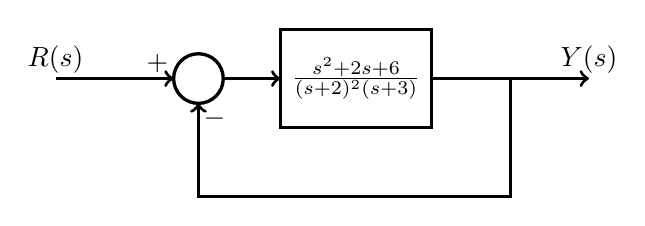
\begin{tikzpicture}[scale=1,inner sep=0pt,outer sep=0pt,very thick,
sysblock/.style={draw,rectangle,inner sep=4pt,minimum width=1.25cm,minimum height=1.25cm,very thick}]

\draw (-2,0) node[draw,circle] (sum1) {$\rule{0pt}{18pt}$};
\draw (0,0) node[sysblock] (G) {$\frac{s^{2}+2s+6}{(s+2)^2(s+3)}$};
\draw[<-] (sum1.180) node[above left=2pt] {$+$} -- ++(-1.5,0) node[above=2pt] {$R(s)$};
\draw[->] (sum1.0) -- (G.180);
\draw[->] (G.0) --  ++(2,0) node[above=2pt] {$Y(s)$};
\draw[->] (G.0) -- ++(1,0) -- ++(0,-1.5) -| (sum1.-90) node[below right=2pt] {$-$};
\end{tikzpicture}
\end{center}
Let the error signal be $e(t)=r(t)-y(t)$. Find

\begin{enumerate}
\renewcommand{\labelenumi}{(\alph{enumi})}
\item The steady state error if the input is $r(t)=10u(t)$ where $u(t)$ is the unit step function.
\item The steady state error if the input is $r(t)=10tu(t)$ where $u(t)$ is the unit step function. 
\end{enumerate}
